\section{not sure yet}

\begin{definition}{CRC-32 nach IEEE 802.3}\\
    Wie können die Standards erreicht werden?\\
    Sicherung der Frames durch den CRC mit Polynom $x^0 + x^1 + ... + x^{32}$
    \begin{itemize}
        \item Minimale Hamming Distanz in Abhängigkeit der Frame-Länge:
        \begin{itemize}
            \item Bei der maximalen Distanz von 12000 Bit ist die minimale Hammingdistanz 4
            \item 3 Fehler können sicher erkannt werden
        \end{itemize}
    \end{itemize}
        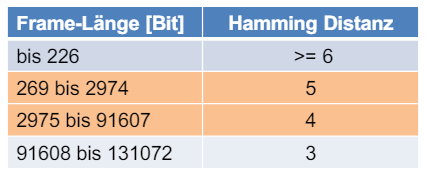
\includegraphics[width=0.5\linewidth]{images/CRC23_bsp.png}
\end{definition}

\begin{formula}{Berechnung der Restfehlerwahrscheinlichkeit}\\
    maximal F=3 Fehler bei einer Übertragung von N=12000 Bits
    $$P_{\leq F, N} = \sum_{t=0}^F \binom{N}{t} \cdot \epsilon^t \cdot (1 - \epsilon)^{N-t}$$
        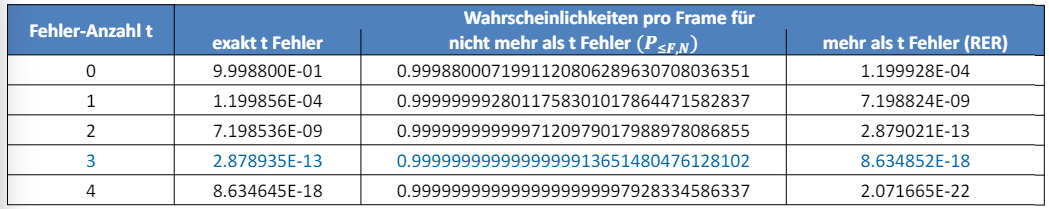
\includegraphics[width=1\linewidth]{images/fehlerwahrscheinlichkeit_berechnen.png}
\end{formula}

\begin{KR}{Worst Case Fehlererkennung für Ethernet}\\
    $5 \cdot 10^{-14}$ unentdeckte Fehler/Frame-Byte, max. BER = $10^{-8}$, max. $F_L$ = 1500 Bytes = 12000 Bit
    \begin{itemize}
        \item Wahrscheinlichkeit für fehlerhafte Frames:
    \end{itemize}
    $$P_{Fehler, Frame} \approx N \cdot p_e$$
    $12000 Bit \cdot 10^{-8} Fehler/Bit = 1.2 \cdot 10^{-4}$ : im Mittel ist jedes 8333. Frame fehlerhaft
    \begin{itemize}
        \item Wahrscheinlichkeit für unerkannte fehlerhafte Frames oberhalb Data Link Layer
    \end{itemize}
    $$RER \leq 1500 \frac{Bytes}{Frame} \cdot 5 \cdot 10^{-14} \frac{Fehler}{Byte} = 7.5 \cdot 10^{-11} \frac{Fehler}{Frame}$$
    ca. jedes 13'000'000'000 Frame ist unerkannt fehlerhaft
    \begin{itemize}
        \item Beispiel Backup 1.5 Tbyte:
    \end{itemize}
    $$1.5 \cdot 10^{12} Byte \cdot 5 \cdot 10^{-14} \frac{Fehler}{Byte} = 0.075 \frac{Fehler}{Backup}$$
    Jedes 13. Backup defekt!
    \begin{itemize}
        \item Beispiel Gigabit-Ethernet:
    \end{itemize}
    $$0.125 \cdot 10^9 \frac{Byte}{s} \cdot 5 \cdot 10^{-14} \frac{Fehler}{Byte} = 6.25 \cdot 10^{-6} \frac{Fehler}{s} = \frac{1 Fehler}{44h}$$
    Alle 44h ein unentdeckter Fehler!
\end{KR}

\subsection*{ICMP}

\begin{definition}{ICMP Meldungstypen - Details}
    \begin{itemize}
        \item Destination Unreachable (Fehler)
        \begin{itemize}
            \item IP-Paket kann nicht zum Ziel gebracht werden
            \item Beispiel: Keine Route zum Ziel-Host vorhanden
        \end{itemize}
        \item Redirect (Optimierung)
        \begin{itemize}
            \item Ein Host H sendet ein IP-Paket an einen ersten Router R1
            \item R1 stellt fest, dass der nächste Router auf dem Weg zum Ziel R2 ist; R2 ist aber im gleichen Netz wie H und R1 (möglicherweise unvollständige Routingtabelle im Host H)
            \item R1 sendet an H eine Redirect-Meldung, damit H Pakete fortan direkt an R2 sendet
        \end{itemize}
        \item Time Exceeded (Fehler)
        \begin{itemize}
            \item Router ändert das TTL-Feld im IP-Header von 1 auf 0
            \item Host hat nicht alle Fragmente erhalten, bevor der Timer abläuft
        \end{itemize}
        \item Parameter Problem: Bad IP Header (Fehler)
        \begin{itemize}
            \item IP Packet Header enthält ungültigen Wert, der nicht verarbeitet werden kann (z.B. nicht existierende IP-Option)
        \end{itemize}
        \item Echo Request/Reply (Information)
        \begin{itemize}
            \item Host sendet Echo-Request, der adressierte Host antwortet mit Echo-Reply; Reply enthält die gleichen Daten wie Request
        \end{itemize}
        \item Timestamp Request/Reply (Information)
        \begin{itemize}
            \item Wie Echo, aber zusätzlich wird die aktuelle Zeit der Hosts ausgetauscht (32-Bit Wert, Millisekunden seit Mitternacht GMT)
        \end{itemize}
    \end{itemize}
\end{definition}

\begin{definition}{Echo Request/Reply Messages}
    Test, ob Host erreichbar ist
    \begin{itemize}
        \item Host antwortet auf Echo Request (Type 8) mit Echo Reply (Type 0), mit gleichem Inhalt wie der Echo Request
    \end{itemize}
    Format
    \begin{itemize}
        \item Identifier: Erlaubt Zuordnung von Reply zu Echo-Request
        \item Sequence Number: Wird innerhalb eines Identifiers jeweils um 1 erhöht
        \item Data: Beliebige Daten, werden vom Empfänger gespiegelt
    \end{itemize}
        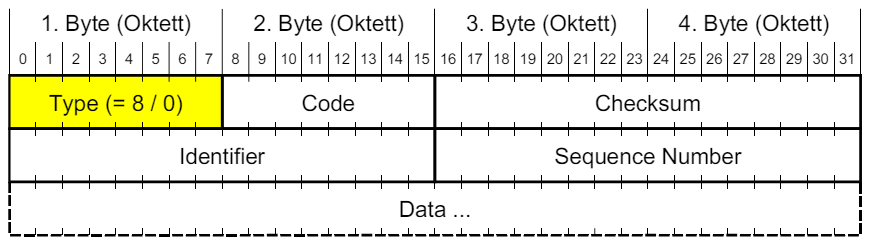
\includegraphics[width=0.75\linewidth]{images/icmp_echorequest.png}\\
    \textbf{ping} verwendet Echo und Echo Reply, um die Erreichbarkeit eines Routers/Hosts zu prüfen; ebenfalls wird die Round-Trip Zeit gemessen\\
        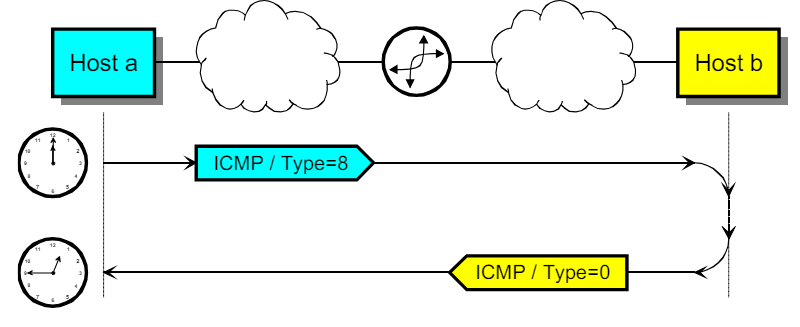
\includegraphics[width=0.75\linewidth]{images/ping.png}
\end{definition}





\begin{definition}{ICMP Time Exceeded}
    \begin{itemize}
        \item \textcolor{blue}{Type = 11}
        \item \textcolor{pink}{unused (must be 0)}
    \end{itemize}
    Wird in diesen 2 Fällen gesendet:
    \begin{itemize}
        \item Router setzt TTL-Feld von 1 auf 0
        \begin{itemize}
            \item Paket wird verworfen und der Absender informiert (Code = 0)
        \end{itemize}
        \item Zielhost kann ein fragmentiertes Paket nicht innerhalb nützlicher Zeit reassemblieren
        \begin{itemize}
            \item Fragmente werden verworfen und der Absender informiert (Code = 1)
        \end{itemize}
    \end{itemize}
    \textbf{traceroute} erlaubt, den Weg zu einem beliebigen Host (oder einem fehlerhaft konfigurierten Router auf diesem Weg) zu finden
    \begin{itemize}
        \item UDP Datagramme an hohe Destination Portnummer (zufällig gewählt, default 33434)
        \item Erstes Datagramm: TTL := 1
        \begin{itemize}
            \item Erster Router setzt TTL auf 0, verwirft Paket und sendet Time Exceeded Message zurück
            \item Erste Router ist bekannt
        \end{itemize}
        \item Nächstes Datagramm: TTL := 2
        \begin{itemize}
            \item Zweiter Router ist bekannt etc...
        \end{itemize}
        \item …
        \item Zielhost kann Zielport nicht erreichen
        \begin{itemize}
            \item Destination Unreachable Message (Code = 1) an Absender
            \item Zielhost ist erreicht
        \end{itemize}
        \item Um die "Entfernung" zu den einzelnen Routern/Zielhosts zu bestimmen, wird zugleich noch die Round-Trip Zeit gemessen
    \end{itemize}
        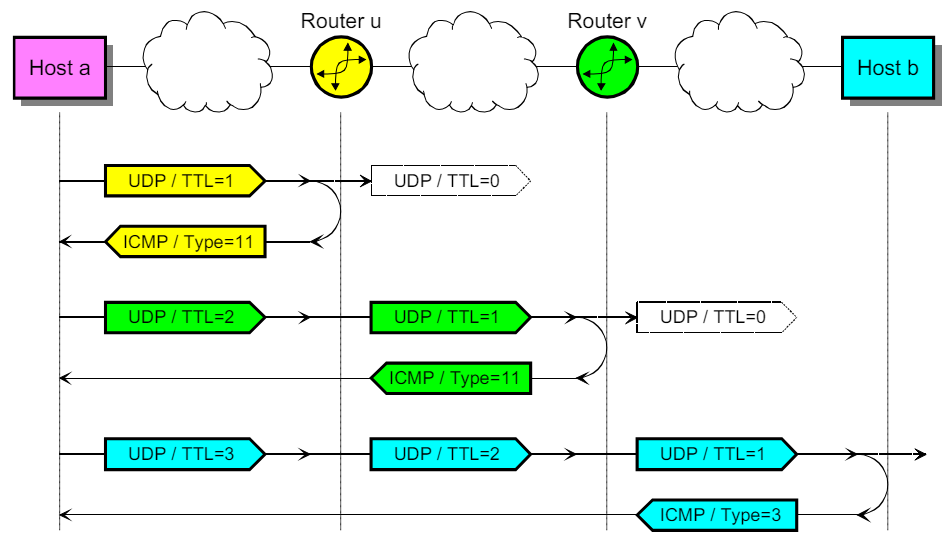
\includegraphics[width=1\linewidth]{images/traceroute.png}
\end{definition}